\chapter*{Dodatek}

\section*{Test}

W związku z awarią sieci teleinformatycznej w Instytucie Sterowania i Techniki Systemów poniższy 
próbny test przeprowadzono 
na skonstruowanym wielokomputerowym systemie WWW za pomocą tylko jednej maszyny komunikującej się z 
systemem za pomocą 10MB huba (firmy IBM). 

Na kolejnych stronach znajdują się wynikowe zestawienia i wykresy próbnego testu wykonanego za 
pomocą oprogramowania Astra LoadTest. Test został wykonany z dziesięcioma wirtualnymi 
użytkownikami\footnote{\emph{Vusers}} (uruchamianymi w kolejności co 15 sek.) poruszającymi się po 
znajdującej się na systemie WWW dokumentacji do serwera Apache (razem dziesięć dowolnie wybranych 
stron). Trwał on 6 min. i 19 sek. Jak widać na rys. \ref{zebrane} łącznie przesłano: $19 915 485$ 
bajtów ze średnią przepustowością na poziomie 52 kb/sek; łącznie $1 925$ trafień (średnio pięć na 
sekundę). Również na rys. \ref{zebrane} znajduje się tabela transakcji wraz ze średnim, minimalnym 
i maksymalnym czasem jej realizacji.

Na rys. \ref{wydajnosc} widać wykres przepustowości serwisu WWW w bajtach na sekundę. Poniżej wykresu 
znajduje się jego charakterystyka wraz z odchyleniem standardowym i medianą.

Kolejny rysunek (rys. \ref{zadania_sekunde}) przedstawia wykres ilości trafień na sekundę 
(charakterystyka wykresu poniżej).

Następny wykres (rys. \ref{pobierana_strona}) przedstawia zależność ilości transakcji od pobranej strony.

Na wykresie (rys. \ref{srednia_odpowiedz}) widać średni czas realizacji transakcji (każdej strony). 
Rys. \ref{zestawienie_odpowiedzi} zawiera zestawienie średnich, najkrótszych i najdłuższych czasów 
realizacji transakcji, a rys. \ref{procentowo} procentowy rozkład ilości transakcji w czasie.

Wykres na rysunku \ref{stron_sekunda} obrazuje ilość pobranych stron na sekundę.

\begin{figure}[h]
\centering
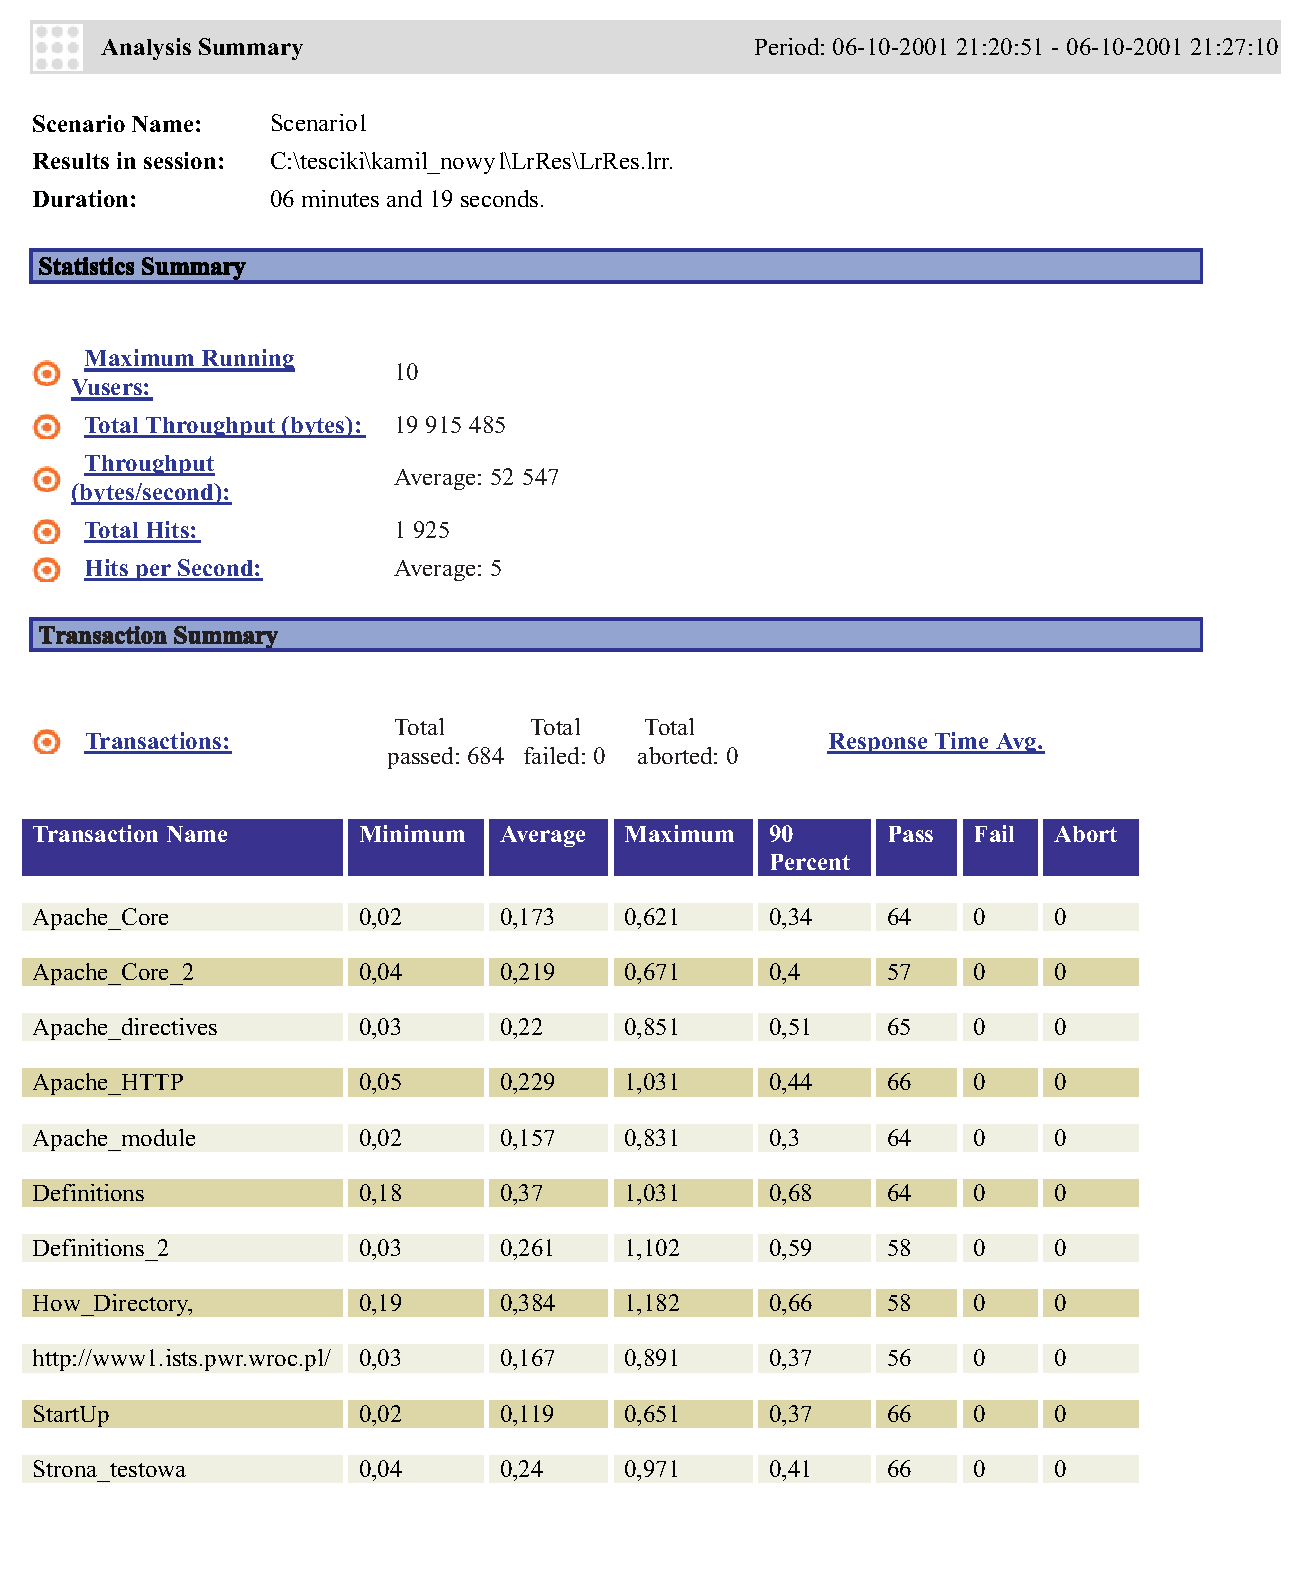
\includegraphics[width=\textwidth]{./rysunki/summary-test.eps}
\caption{Zebrane informacje o przebiegu testu}
\label{zebrane}
\end{figure}
\begin{figure}[h]
\centering

\includegraphics[width=4.5in]{./rysunki/raport1calybokiem.eps}
\caption{Wydajność wielokomputerowego systemu WWW}
\label{wydajnosc}
\end{figure}
\begin{figure}[h]
\centering

\includegraphics[width=4.5in]{./rysunki/raport2calybokiem.eps}
\caption{Ilość realizacji żądań na sekundę}
\label{zadania_sekunde}
\end{figure}
\begin{figure}[h]
\centering

\includegraphics[width=4.5in]{./rysunki/rapor3calybokiem.eps}
\caption{Ilość transakcji w zależności od pobieranej strony}
\label{pobierana_strona}
\end{figure}
\begin{figure}[h]
\centering
\includegraphics[width=\textwidth]{./rysunki/raport4calybokiem.eps}
\caption{Średni czas odpowiedzi}
\label{srednia_odpowiedz}
\end{figure}
\begin{figure}[h]
\centering
\includegraphics[width=4.5in]{./rysunki/raport7calybokiem.eps}
\caption{Zestawienie odpowiedzi w zależności od pobieranej strony}
\label{zestawienie_odpowiedzi}
\end{figure}
\begin{figure}[h]
\centering
\includegraphics[width=\textwidth]{./rysunki/raport9calybokiem.eps}
\caption{Czas odpowiedzi transakcji -- udział procentowy}
\label{procentowo}
\end{figure}
\begin{figure}[h]
\centering
\includegraphics[width=\textwidth]{./rysunki/raport10calybokiem.eps}
\caption{Czas odpowiedzi transakcji -- rozkład}
\label{odpowiedz_transakcji_rozklad}
\end{figure}
\begin{figure}[h]
\centering

\includegraphics[width=4.5in]{./rysunki/raport11calybokiem.eps}
\caption{Liczba stron na sekundę}
\label{stron_sekunda}
\end{figure}


